\documentclass{beamer}

\mode<presentation> {

% The Beamer class comes with a number of default slide themes
% which change the colors and layouts of slides. Below this is a list
% of all the themes, uncomment each in turn to see what they look like.

%\usetheme{default}
%\usetheme{AnnArbor}
%\usetheme{Antibes}
%\usetheme{Bergen}
%\usetheme{Berkeley}
%\usetheme{Berlin}
%\usetheme{Boadilla}
\usetheme{CambridgeUS}
%\usetheme{Copenhagen}
%\usetheme{Darmstadt}
%\usetheme{Dresden}
%\usetheme{Frankfurt}
%\usetheme{Goettingen}
%\usetheme{Hannover}
%\usetheme{Ilmenau}
%\usetheme{JuanLesPins}
%\usetheme{Luebeck}
%\usetheme{Madrid}
%\usetheme{Malmoe}
%\usetheme{Marburg}
%\usetheme{Montpellier}
%\usetheme{PaloAlto}
%\usetheme{Pittsburgh}
%\usetheme{Rochester}
%\usetheme{Singapore}
%\usetheme{Szeged}
%\usetheme{Warsaw}

% As well as themes, the Beamer class has a number of color themes
% for any slide theme. Uncomment each of these in turn to see how it
% changes the colors of your current slide theme.

%\usecolortheme{albatross}
%\usecolortheme{beaver}
%\usecolortheme{beetle}
%\usecolortheme{crane}
%\usecolortheme{dolphin}
%\usecolortheme{dove}
%\usecolortheme{fly}
%\usecolortheme{lily}
%\usecolortheme{orchid}
%\usecolortheme{rose}
%\usecolortheme{seagull}
%\usecolo rtheme{seahorse}
%\usecolortheme{whale}
%\usecolortheme{wolverine}

%\setbeamertemplate{footline} % To remove the footer line in all slides uncomment this line
%\setbeamertemplate{footline}[page number] % To replace the footer line in all slides with a simple slide count uncomment this line

%\setbeamertemplate{navigation symbols}{} % To remove the navigation symbols from the bottom of all slides uncomment this line
}

\usepackage{graphicx} % Allows including images
\usepackage{booktabs} % Allows the use of \toprule, \midrule and \bottomrule in tables
%\usepackage{german}
\usepackage{braket}
\usepackage{bbold}
\usepackage[utf8]{inputenc}
\usepackage{wasysym}
\usepackage{hyperref}
\usepackage{tcolorbox}
\usepackage{ragged2e}

\setbeamertemplate{caption}[numbered]

%----------------------------------------------------------------------------------------
%	TITLE PAGE
%----------------------------------------------------------------------------------------

\title[HPC 1b]{High Performance Computing 1b \\
Parallelization of a 2D Hydro Solver} % The short title appears at the bottom of every slide, the full title is only on the title page

\author[Hertig, Radonic]{Remo Hertig\\
Stephan Radonic} % Your name
\institute[UZH] % Your institution as it will appear on the bottom of every slide, may be shorthand to save space
{
University of Zurich
}
\date{\today} % Date, can be changed to a custom date

\begin{document}

\begin{frame}
\titlepage % Print the title page as the first slide
\end{frame}

%\begin{frame}
%\frametitle{Overview} % Table of contents slide, comment this block out to remove it
%\tableofcontents % Throughout your presentation, if you choose to use \section{} and \subsection{} commands, these will automatically be printed on this slide as an overview of your presentation
%\end{frame}

%----------------------------------------------------------------------------------------
%	PRESENTATION SLIDES
%----------------------------------------------------------------------------------------

%------------------------------------------------
%\section{HYDRO Parallelization} % Sections can be created in order to organize your presentation into discrete blocks, all sections and subsections are automatically printed in the table of contents as an overview of the talk
%------------------------------------------------
%\subsection{Introduction}
%\subsection{Parallelization strategy}
%\subsection{Serial vs. Parallel Processing}
%\subsection{Scaling and Speedup}
%\subsection{High resolution example}
%
%
%
\begin{frame}
\frametitle{Introduction and physics}
\justify
\small{
Our task was to parallelize an existing C code, originally written by Prof. Romain Teyssier in Fortran, which solves the Euler equations in 2D using a Godunov scheme. The euler equations in conservation form are 
\begin{equation}
\partial_t
\begin{pmatrix} \rho    \\ \rho \mathbf{u}\\0\end{pmatrix}+\nabla\cdot\begin{pmatrix} \rho\mathbf{u}    \\ \rho\mathbf{u}\otimes\mathbf{u}+p\mathbf{I}\\ \mathbf{u}\end{pmatrix} = 0
\end{equation}
This set of equations describes the flow of a gas basically stating the momentum, mass and energy conservation. A hyperbolic PDE in conservation law form is generally represented as
\begin{equation}
\partial_t\mathbf{U} + \nabla\cdot\mathbf{F(U)} = 0
\label{eq:bb}
\end{equation}
Discretization on a grid yields
\begin{equation}
\mathbf{U}^{n+1}_i=\mathbf{U^n_i}+\frac{\Delta x}{\Delta t}(\mathbf{F_{i-1/2}}-\mathbf{F_{i+1/2}})
\label{eq:bc}
\end{equation}
where $\mathbf{F_{i\pm1/2}}$ are the fluxes at the cell boundaries, the Godunov scheme uses various approximations for $\mathbf{F_{i\pm1/2}}$, depending on the specific variation of the method, e.g upwind scheme, lax-friedrich, ... \\
}


\end{frame}

%
%
%
\begin{frame}
\frametitle{Parallelization: Strategy}

We implemented a symmetric vertical domain decomposition\footnote{ 
\emph{Restriction: $width\in W,~~W=\{k\cdot n_{proc}|k\in\mathbb{N}\}$ } } and used nonblocking MPI communication to share ghost cells.\\
\vspace{2mm}
Since the resulting data output is massive (\textasciitilde{}600Mb for a 10M grid per step) it is currently unpractical to store the results from every step. Therefore we opted for a lower writing frequency. This allows us to implement the "write-to-disk" part in a rather sub-optimal way: MPI\_Gather to the master. However the performance impact of this strategy is negligible with sparing data writing.\\
\vspace{2mm}
Further we minimized memory reallocations and reused buffers to improve data locality for exploiting the cache. \\

\end{frame}

\begin{frame}
\frametitle{Exploratory runs I}
Investigating gridsize memory usage on cache trashing for  on a 1/socket \footnote{aprun -N 1 --ntasks=1 -S 1 -ss --cpu\_bind=sockets} and a 12/socket run.\footnote{aprun -N 1 --ntasks=1 -S 12 -ss -m plane=24:block --cpu\_bind=cores} with y=1000 \footnotesize{[t/mp = time to calculate 1m cells]}

\begin{minipage}[1\textheight]{\textwidth}
\begin{columns}[T]

\begin{column}{0.5\textwidth}
\begin{figure}
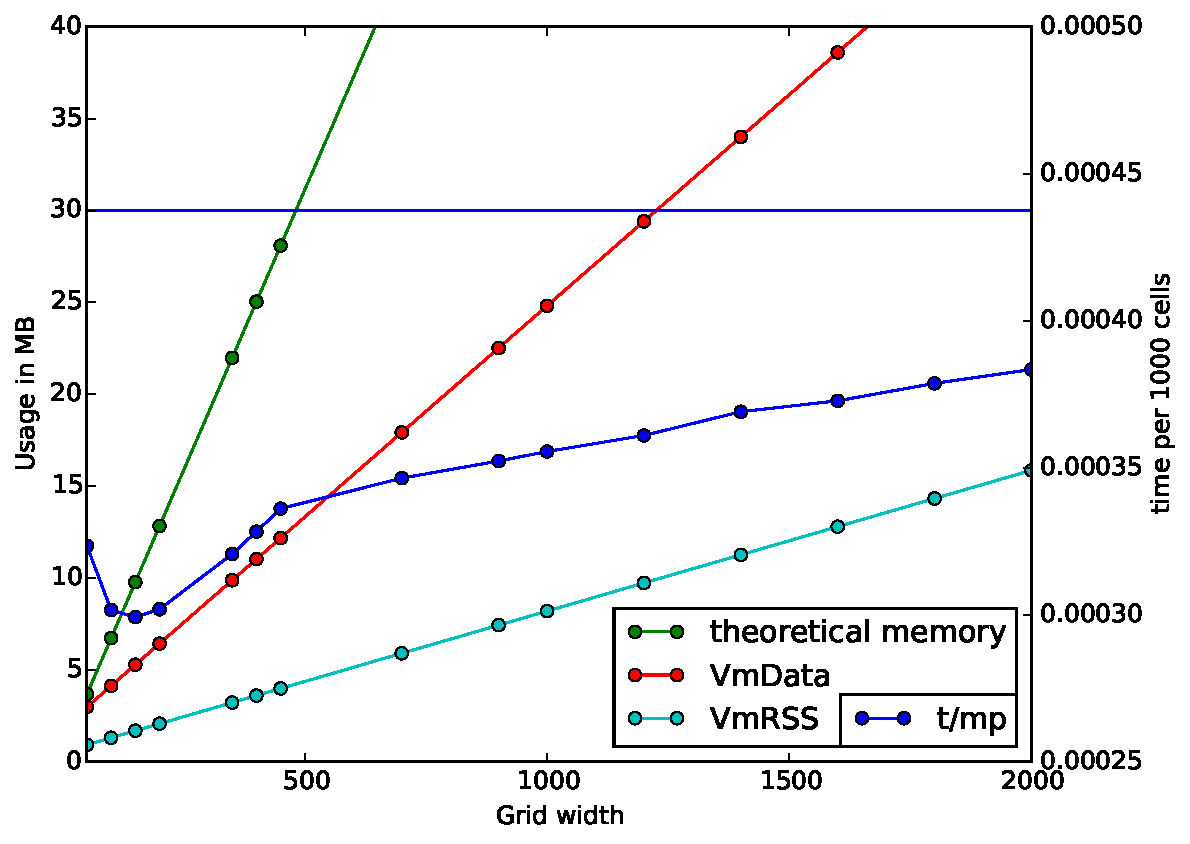
\includegraphics[width=6.15cm]{T2.pdf}
\caption{ 2 processes per node}
\end{figure}

\end{column}


\begin{column}{0.5\textwidth}
\begin{figure}
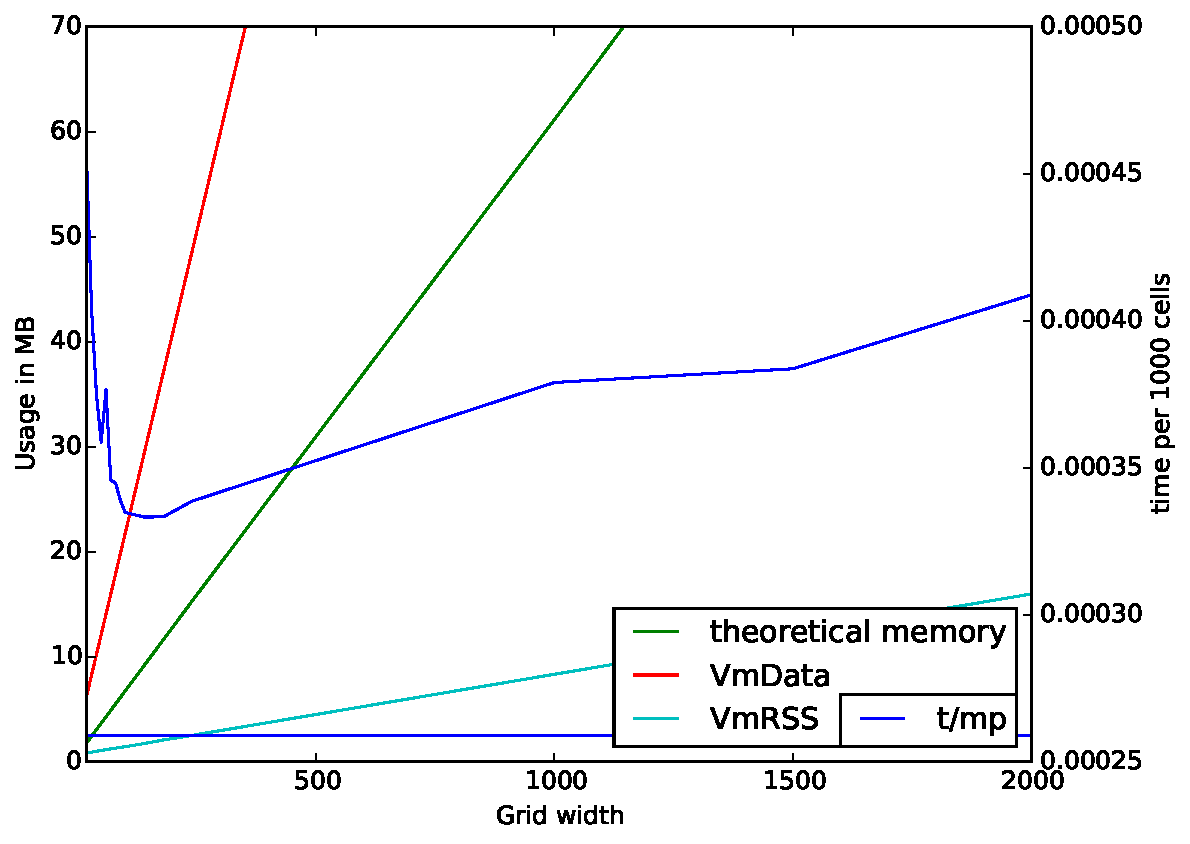
\includegraphics[width=6.15cm]{T12.pdf}
\caption{24 processes per node}
\end{figure}
\end{column}
\end{columns}
\end{minipage}



\end{frame}


%
%
%
\begin{frame}
\frametitle{Exploratory runs II}

Theoretical memory usage was predicted through analyzing allocations throughout the code with: $m(x_{width},y_{height})=\begin{cases}
y>x & y(4x+82)\\
y<x & x(4y+66)+16y\end{cases}$ \\
VmData, VmRSS: actual measures\footnote{see \emph{man proc}}. We can see a lower computing time per cell when at least the working set fits into the LLC=30MB\footnote{Intel® Xeon® E5-2690 v3}\\ The high memory usage of the 12/socket case is probably due to MPI overhead.
 
Therefore we predict an optimal performance using a working set of around $150\times1000$ per MPI process.

\end{frame}
%
%
%
\begin{frame}
\frametitle{Parallelization: Speedup}
\begin{minipage}[1\textheight]{\textwidth}
\begin{columns}[T]
\begin{column}{0.5\textwidth}
\vspace{5mm}
\justify

We compare the average time step durations up to approximately 1536 parallel processes with the time of the mono version.

The predicted speedup according to Amdahl's law was estimated based on the measured speedup (s) for a given number of processes (n) with: $P_{predicted}=\frac{\frac{1}{s}-1}{\frac{1}{n}-1}$


We explain the super-linear speedup with our choice of parameters (grid size, nProc) to exploit caches optimally.



\end{column}
\begin{column}{0.5\textwidth}
\begin{figure}
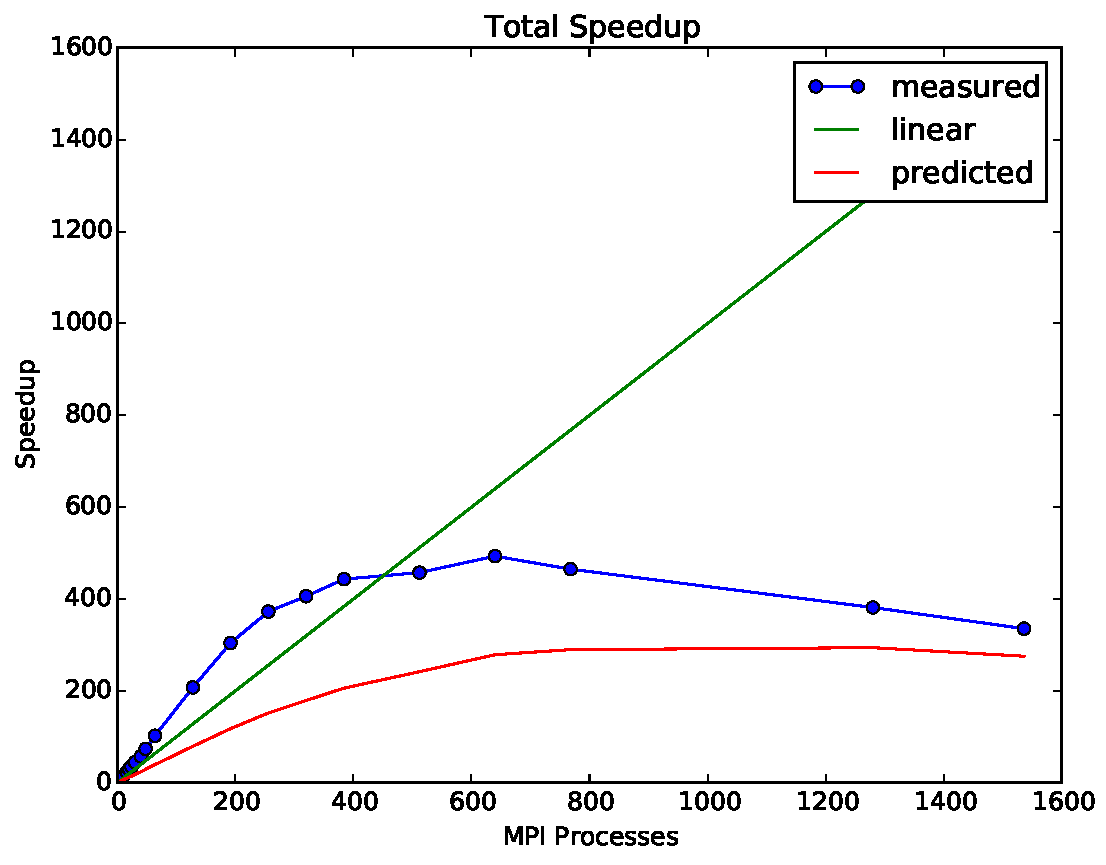
\includegraphics[width=6cm]{speedup.pdf}
\caption{Speedup on a grid of $20480\times 492$}

\end{figure}
\end{column}
\end{columns}
\end{minipage}
\end{frame}

%
%
%
\begin{frame}
\frametitle{Parallelization: Strong Scaling}

\begin{minipage}[1\textheight]{\textwidth}
\begin{columns}[T]
\begin{column}{0.7\textwidth}
\begin{figure}
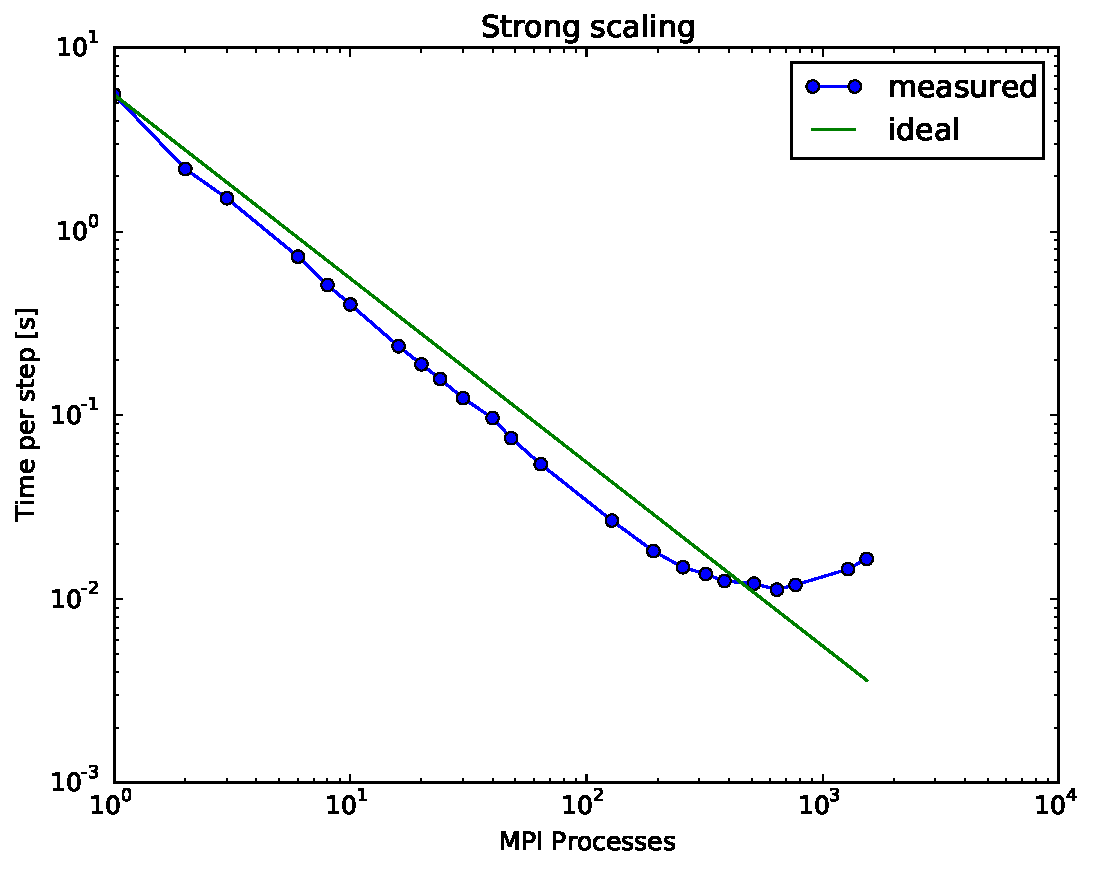
\includegraphics[width=6.55cm]{strongscale.pdf}
\caption{grid of $20480\times 492$ for 1 to 1536 processes. Time step decreasing from 4.65 to 0.009}
\end{figure}
\end{column}

\begin{column}{0.3\textwidth}
\justify
We can see that with $>512$ processors the MPI communication overhead is having a heavy impact on the performance.


\end{column}
\end{columns}
\end{minipage}


\end{frame}

%
%
%
\begin{frame}
\frametitle{Output image I}
\justify
To use the provided computing resources economically we constrained ourself to a $3360\times510$ grid with 112 MPI processes on 5 nodes (run time: 1:02:21)\\

\vspace{-5mm}
\begin{figure}

\includegraphics[width=12.2cm]{7c.png}
\caption{$t=461$}
\end{figure}

\vspace{-7mm}
\begin{figure}
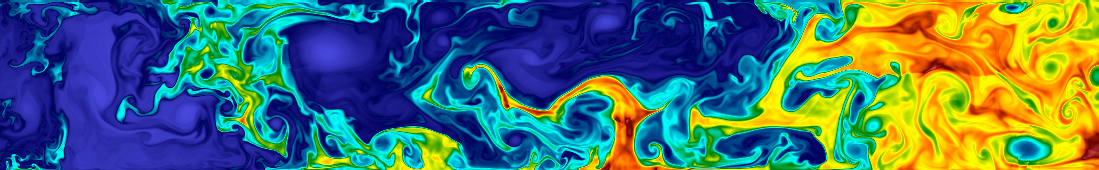
\includegraphics[width=12.2cm]{10c.png}
\caption{$t=1772$}
\end{figure}



\end{frame}
%
%
%
\begin{frame}
\frametitle{Output image II}

\begin{figure}
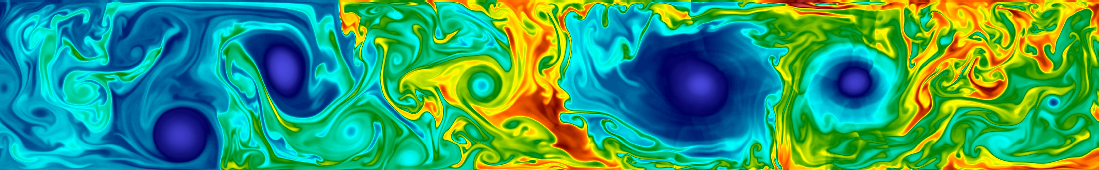
\includegraphics[width=12.2cm]{13c.png}
\caption{$t=4543$}
\end{figure}

\begin{figure}
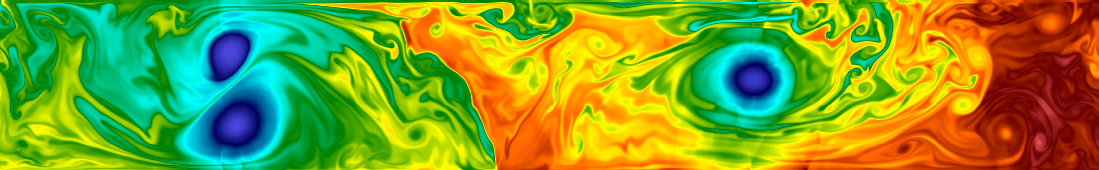
\includegraphics[width=12.2cm]{17c.png}
\caption{$t=9230$}
\end{figure}



\end{frame}

%
%
%
\end{document} 
